\chapter{Larger Gantt Diagram}

\begin{figure}[H]
    \centering
    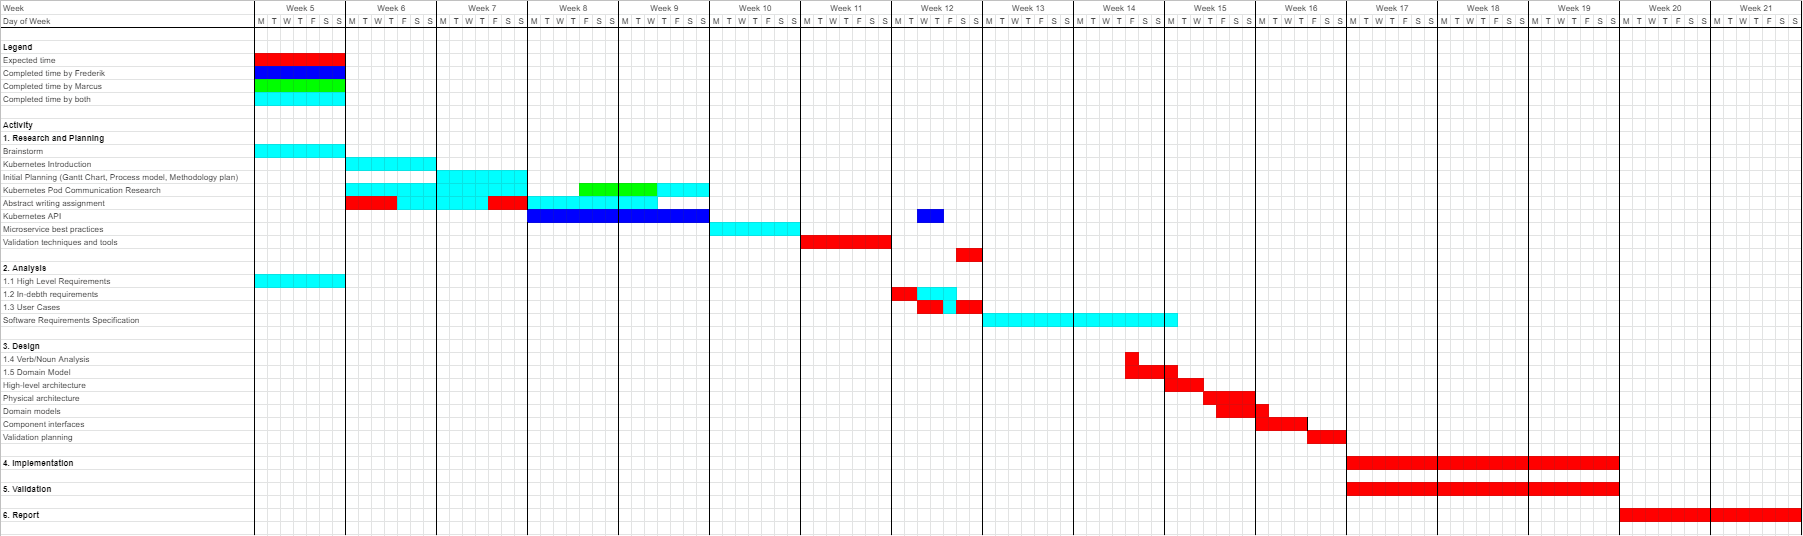
\includegraphics[width=0.8\textheight,angle=90]{Pictures/Gantt.png}
    \caption{Larger version of the figure shown in the Methodology and Process chapter. The picture is still not very clear, but the image is too large and is not of particular importance.}
    \label{fig:ganttLarge}
\end{figure}

\newpage
\chapter{Full size Odin deployment design}

\begin{figure}[h]
    \centering
    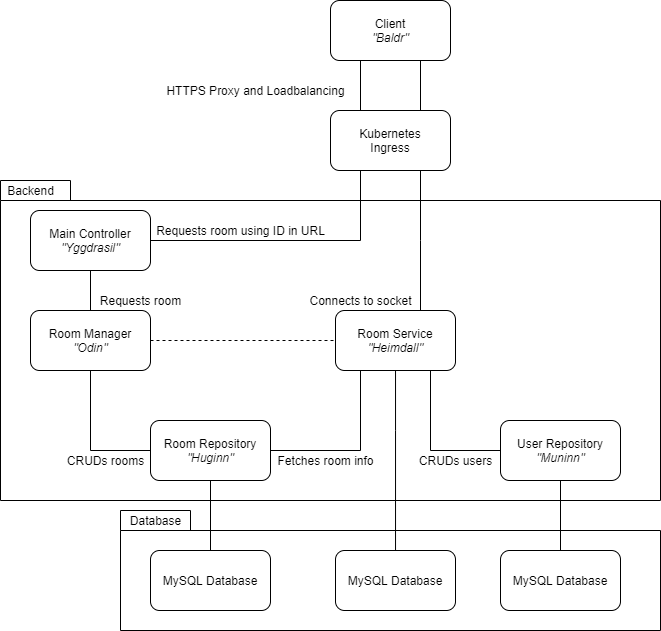
\includegraphics[width=\textwidth]{Pictures/Odin Final Design.png}
    \caption{The full sized image of the Odin deployment displayed in the Design chapter.}
    \label{fig:odinDesignFullSized}
\end{figure}

\newpage
\chapter{Full size Vili deployment design}

\begin{figure}[h]
    \centering
    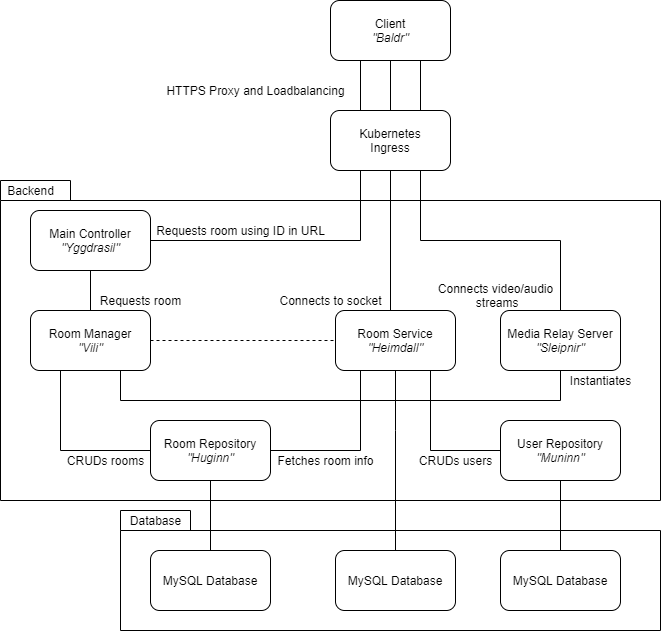
\includegraphics[width=\textwidth]{Pictures/Vili Final Design.png}
    \caption{The full sized image of the Vili deployment displayed in the Design chapter.}
    \label{fig:viliDesignFullSized}
\end{figure}

\newpage
\chapter{Initially proposed design, part 1/2}

\begin{figure}[H]
    \centering
    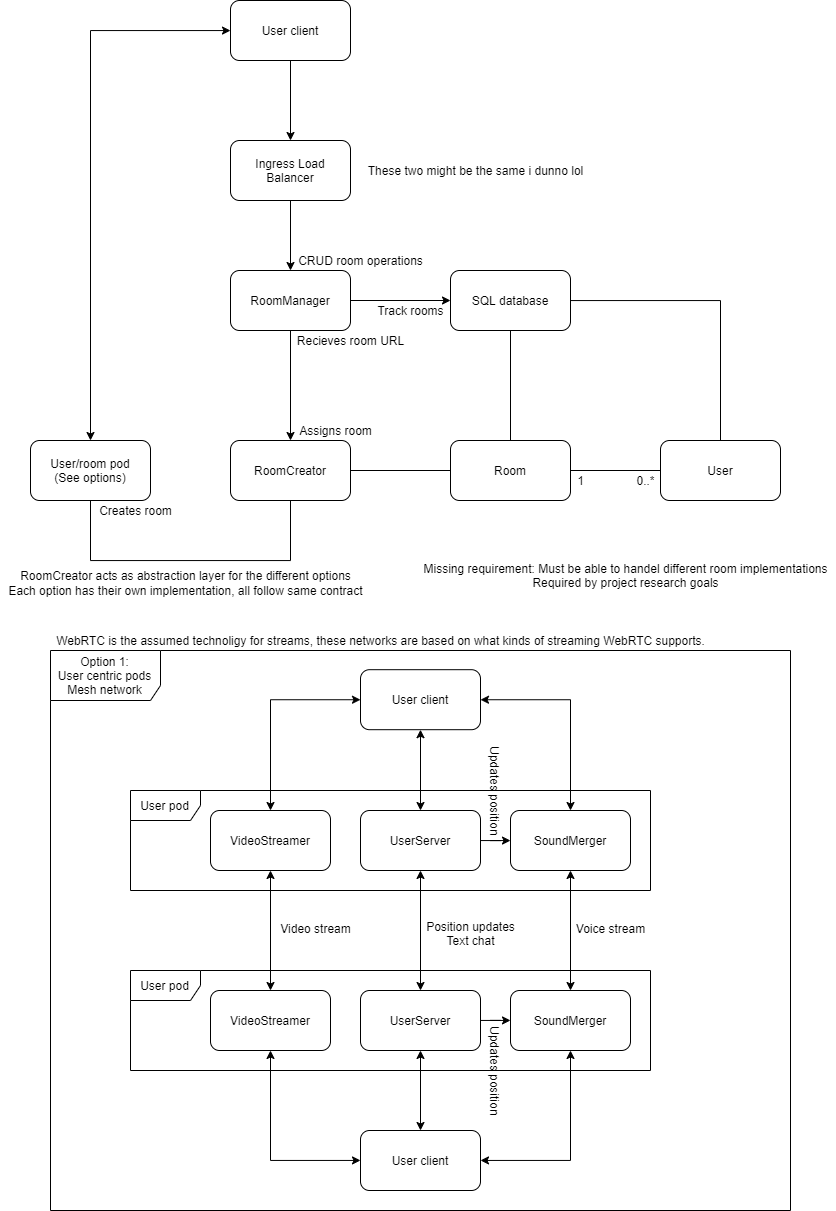
\includegraphics[width=0.8\textwidth]{Pictures/InitialDesignP1.png}
    \caption{The initially proposed design of the system post-analysis. Notice the much more complex room designs in the panel marked as Option 1, as well as option 2 and 3 displayed in \ref{fig:initialdesign2}. This is the general area of the design that was heavily simplified. The upper part of the figure displays the initial design of shared components, many of which survived the changes, such as but not limited to the RoomManager which became Yggdrasil, the RoomCreator which became Odin/Vili, and the user/room pod which became Heimdall.}
    \label{fig:initialdesign1}
\end{figure}

\chapter{Initially proposed design, part 2/2}

\begin{figure}[H]
    \centering
    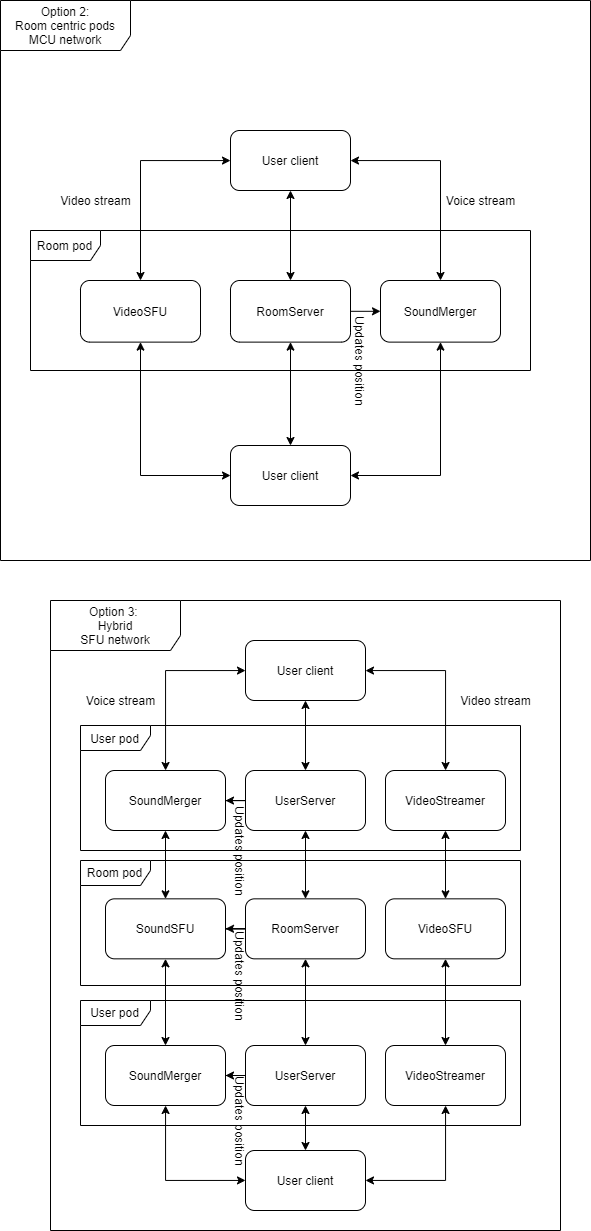
\includegraphics[width=0.60\textwidth]{Pictures/InitialDesignP2.png}
    \caption{The second part of the initially proposed design, displaying two other room design variations. Option 2 displayed here is closest to the final design, with RoomServer being roughly equivalent to Heimdall, and SoundMerger and VideoSFU being rougly equivalent to Sleipnir.}
    \label{fig:initialdesign2}
\end{figure}


\newpage
\chapter{Use Cases created in the analysis phase of the project}

\begin{figure}[H]
    \centering
    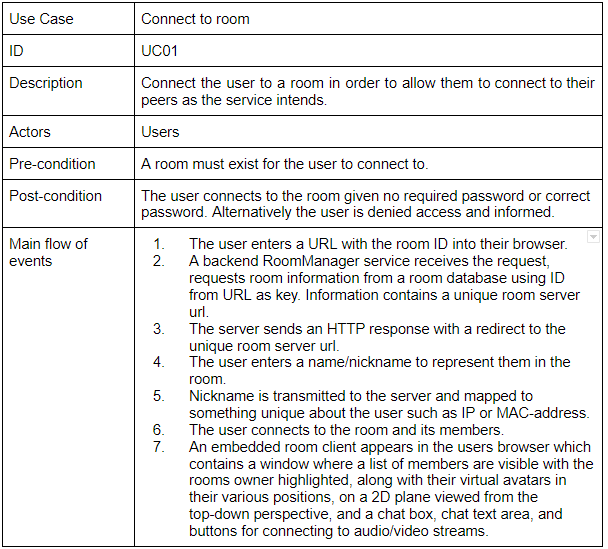
\includegraphics[width=0.65\textwidth]{Pictures/UseCaseConnect.png}
    \caption{This Use Case illustrates the flow of events of when a user connects to a room.}
    \label{fig:usecase1}
\end{figure}

\begin{figure}[H]
    \centering
    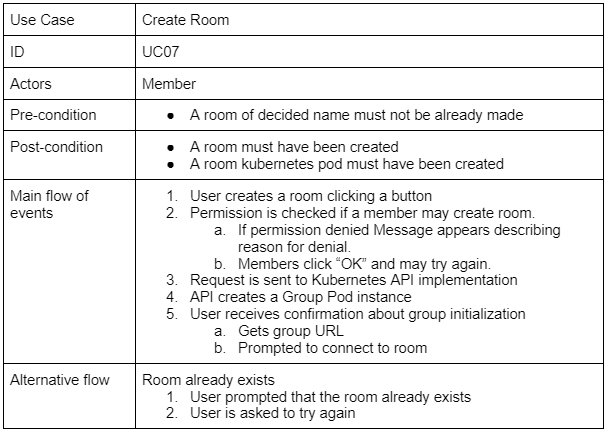
\includegraphics[width=0.65\textwidth]{Pictures/UseCaseCreateRoom.png}
    \caption{This Use Case illustrates the flow of events of when a user connects creates a room.}
    \label{fig:usecase2}
\end{figure}

\newpage

\begin{figure}[H]
    \centering
    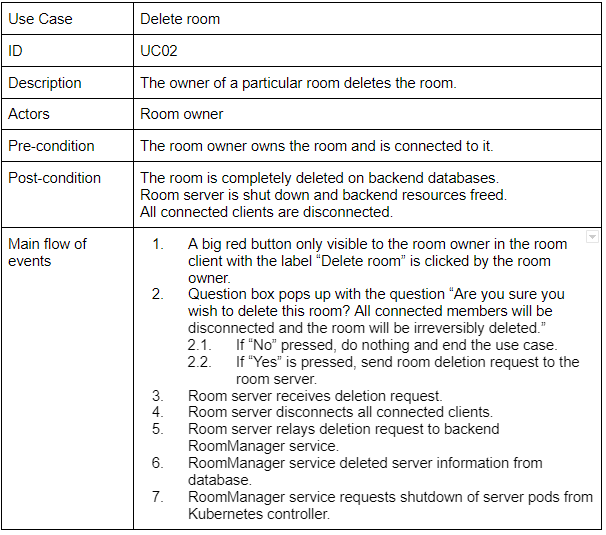
\includegraphics[width=0.65\textwidth]{Pictures/UseCaseDeleteRoom.png}
    \caption{This Use Case illustrates the flow of events of when a user deletes a room.}
    \label{fig:usecase3}
\end{figure}

\begin{figure}[H]
    \centering
    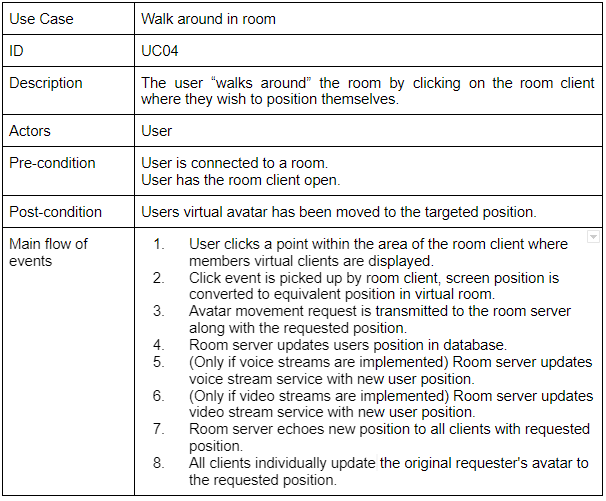
\includegraphics[width=0.65\textwidth]{Pictures/UseCaseMove.png}
    \caption{This Use Case illustrates the flow of events of when a user moves around the room canvas.}
    \label{fig:usecase4}
\end{figure}

\newpage

\begin{figure}[H]
    \centering
    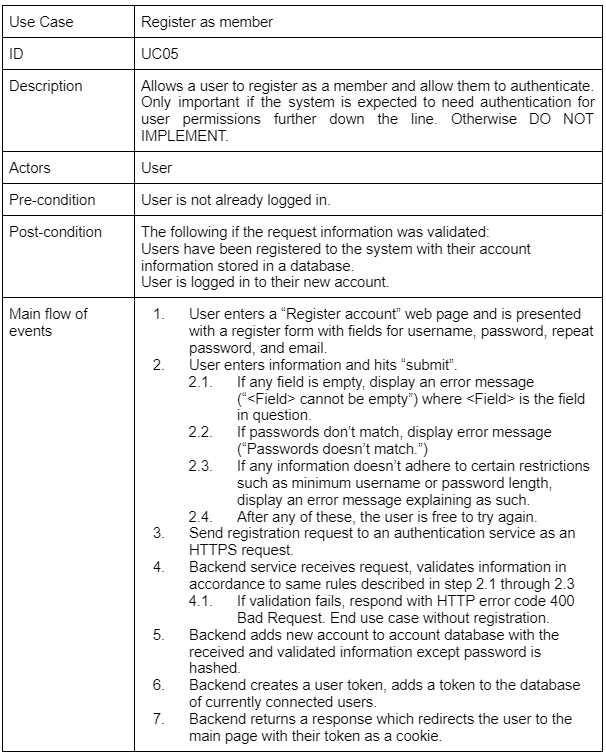
\includegraphics[width=0.65\textwidth]{Pictures/UseCaseRegisterMember.png}
    \caption{This Use Case illustrates the flow of events of when a user registers as a member. This is functionality never made it to the final product.}
    \label{fig:usecase5}
\end{figure}

\begin{figure}[H]
    \centering
    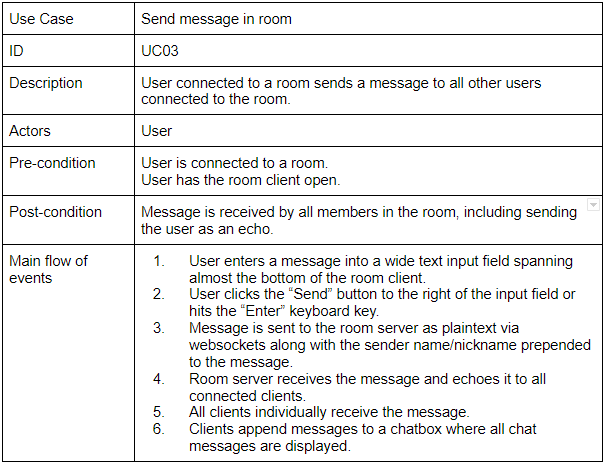
\includegraphics[width=0.65\textwidth]{Pictures/UseCaseSendMessage.png}
    \caption{This Use Case illustrates the flow of events of when a user sends a message to the room it is connected to.}
    \label{fig:usecase6}
\end{figure}

\newpage

\begin{figure}[H]
    \centering
    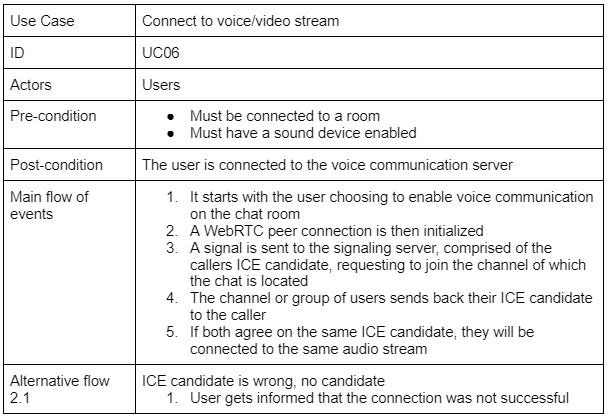
\includegraphics[width=0.65\textwidth]{Pictures/UseCaseWebRTC.png}
    \caption{This Use Case illustrates the flow of events of when a user tries to connect to another user with audio and video through WebRTC.}
    \label{fig:usecase7}
\end{figure}

\newpage
\chapter{Artillery Stress Test Summaries}
\begin{lstlisting}[language=text]
Room Repository Stress Test

All virtual users finished
Summary report @ 16:21:31(+0200) 2021-05-31
  Scenarios launched:  33554
  Scenarios completed: 33548
  Requests completed:  33548
  Mean response/sec: 42.97
  Response time (msec):
    min: 26
    max: 4801
    median: 32
    p95: 39
    p99: 56
  Scenario counts:
    Get rooms: 33554 (100%)
  Codes:
    200: 33548
  Errors:
    ETIMEDOUT: 6

User Repository Stress Test

All virtual users finished
Summary report @ 18:46:32(+0200) 2021-05-31
  Scenarios launched:  33658
  Scenarios completed: 33658
  Requests completed:  33658
  Mean response/sec: 43.1
  Response time (msec):
    min: 32
    max: 289
    median: 35
    p95: 42
    p99: 48
  Scenario counts:
    Get users: 33658 (100%)
  Codes:
    200: 33658

Socket Server Stress Test

All virtual users finished
Summary report @ 18:50:25(+0200) 2021-05-31
  Scenarios launched:  120
  Scenarios completed: 120
  Requests completed:  517
  Mean response/sec: NaN
  Response time (msec):
    min: 0.1
    max: 2.3
    median: 0.1
    p95: 0.2
    p99: 0.3
  Scenario counts:
    Busy boys: 19 (15.833%)
    Lurker: 84 (70%)
    A mostly quiet user: 17 (14.167%)
  Codes:
    0: 517
  engine.socketio.emit: 517
\end{lstlisting}

